%-- einleitung

\section{Einführung}

\subsection{Ziele}

Das Ziel dieses Projektes ist es zum einen ein System zu entwickeln, das die Möglichkeiten von Genetischen Algorithmen am Beispiel des Travelling-Salesman-Problem, demonstriert.
Darüber hinaus soll untersucht werden welche Stellschrauben der Genetischen Algorithmen die Resultate inwieweit positiv oder negativ beeinflussen.

\subsection{Genetische Algorithmen}

\begin{figure}[H]
\centering
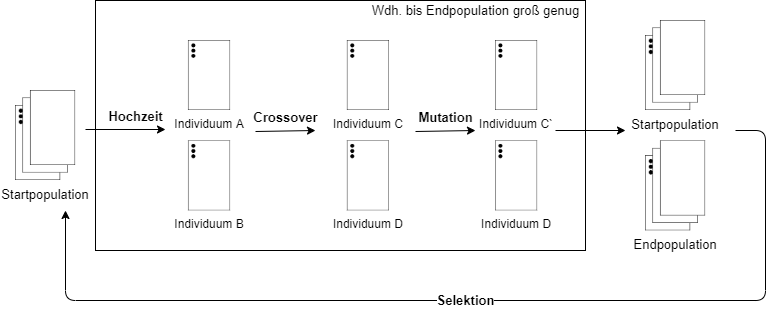
\includegraphics[width=1\textwidth]{img/Vortrag/Genetic_Algorithm.png}
\caption{Überblick Genetischer Algorithmus}
\label{fig:genetic_algorithm}
\end{figure}

\subsection{Travelling Salesman Problem}

\begin{figure}[H]
\centering

\includegraphics[width=0.5\textwidth]{img/Vortrag/TSP_Deutschland.png}
\caption{Travelling Salesman Problem}
\label{fig:TSP}
\end{figure}

\subsection{Struktur der Arbeit}

%--